\LevelOneTitle{流体动力学积分方程分析}

\begin{tip}
	本章中雷诺输运公式和原始形式的连续方程、能量方程和动量方程的数学表达式均不需要掌握,重点是理解物理意义和用控制体描述系统的研究思想,以及熟练掌握解题方法(只掌握做题方法当然也可以)。本章考计算题的概率非常大。
\end{tip}

\LevelTwoTitle{系统和控制体}

\begin{definition}[系统]
	某一确定流体质点集合的总体,与外界无质量交换,随流体质点运动,边界形状、包围空间大小随流体质点运动而变化。
\end{definition}

\begin{definition}[控制体]
	流场中某一确定的空间区域,与外界有质量交换,空间位置相对参照系不变,有确定的边界形状和包围空间大小。
\end{definition}

\LevelTwoTitle{*雷诺输运公式}

\begin{equation}
	\dfrac{\mathrm{D} \varPhi_{\text{sys}}}{\mathrm{D} t} = \pdv{t} \int_{\text{CV}} \phi \dd{\tau} + \int_{\text{CS}} \phi \vec{V} \cdot \vec{n} \dd{S}
\end{equation}

物理意义

\begin{enumerate}
	\item $\dfrac{\mathrm{D} \varPhi_{\text{sys}}}{\mathrm{D} t}$表示系统物理量$\varPhi_{\text{sys}}$随时间的变化率;
	\vskip 0.1cm
	\item $\displaystyle \pdv{t} \int_{\text{CV}} \phi \dd{\tau}$表示控制体物理量$\varPhi$对时间的变化率,反映流场的非定常性;
	\vskip 0.1cm
	\item $\displaystyle \int_{\text{CS}} \phi \vec{V} \cdot \vec{n} \dd{S}$表示控制体物理量$\varPhi$流出控制体的净流率,反映流场的非均匀性,体现系统位置、体积随时间改变。
	\item 整个公式是欧拉方法下采用与控制体相关的物理量描述系统的物质导数。
\end{enumerate}

\begin{tip}
	本质上,雷诺输运公式(积分形式,研究系统物理量和控制体物理量之间的关系)和物质导数公式(微分形式,研究流体质点物理量和空间点物理量之间的关系)是等价的。
\end{tip}

\LevelTwoTitle{控制方程}

\LevelThreeTitle{连续方程}

\begin{equation}
	\dfrac{\mathrm{D} m}{\mathrm{D} t} = \pdv{t} \int_{\text{CV}} \rho \dd{\tau} + \int_{\text{CS}} \rho \vec{V} \cdot \vec{n} \dd{S} 
\end{equation}

连续方程依然是质量守恒定律的应用,每一项的物理意义可以依照雷诺输运公式的解释写出,对于控制体来说,单位时间CV内流体质量增加与净流出CV的流体质量流量之和为0,可以回顾第\ref{3.5}节中的欧拉连续性原理。

\textbf{计算题中只需要掌握}在均布、定常条件下的简化形式:
\begin{equation}
	\begin{split}
		\dot{m} &= \rho V A = \text{const} \\
		Q &= V A = \text{const}
	\end{split}
\end{equation}

\LevelThreeTitle{能量方程}

\begin{equation}
	\dfrac{\mathrm{D} E}{\mathrm{D} t} = \dot{Q} + \dot{W} = \pdv{t} \int_{\text{CV}} \rho e \dd{\tau} + \int_{\text{CS}} \rho e \vec{V} \cdot \vec{n} \dd{S} 
\end{equation}

\textbf{计算题中只需要掌握}总流伯努利方程:

\begin{equation}
	z + \dfrac{p}{\rho g} + \dfrac{\alpha \overline{V}^2}{2 g} = \text{const}
\end{equation}

其中,$\alpha$为动能修正系数,反映过流断面速度分布不均匀性,在本章计算题中取1即可,实际数学表达式为
\begin{equation}
	\alpha = \dfrac{\displaystyle \int_{A} V^3 \dd{A}}{\overline{V}^3 A}
\end{equation}

总流伯努利方程的适用条件
\begin{enumerate}
	\item 理想不可压;
	\item 定常;
	\item 质量力有势且只有重力;
	\item 两过流断面必须是缓变流过流断面;
	\item 两过流断面间无能量输入输出。
\end{enumerate}

\begin{definition}[缓变流]
	流线近似于互相平行的直线的流动称为缓变流,缓变流过流断面上流体重力势能和压力能之和为常数,动压分布和静压分布相同,即
	\begin{equation}
		z + \dfrac{p}{\rho g} = \text{const}
	\end{equation}
\end{definition}

\LevelThreeTitle{动量方程}

\begin{equation}
	\sum \vec{F} = \pdv{t} \int_{\text{CV}} \rho \vec{V} \dd{\tau} + \int_{\text{CS}} \rho \vec{V} \vec{V} \cdot \vec{n} \dd{S} 
\end{equation}

\textbf{计算题中只需要掌握}

\begin{equation}
	\sum \vec{F} = \sum \qty(\dot{m}_i \vec{V}_i)_{\text{out}} - \sum \qty(\dot{m}_i \vec{V}_i)_{\text{in}}
\end{equation}

其中,$\dot{m} = \rho V A$。动量正负号规则是:与坐标方向一致为正,相反为负。

\LevelTwoTitle{例题练习}

\begin{example}
	如图,一圆盘中心有一锐边圆孔,速度为$V$的水射流撞击在圆盘中心,通过圆盘中心孔的射流速度也是$V$。试求需施加多大的力才能保持圆盘在空间位置不变。设$V = 5$ m/s,$D = 100$ mm,$d = 20$ mm。
	
	\begin{figure}[H]
		\centering
		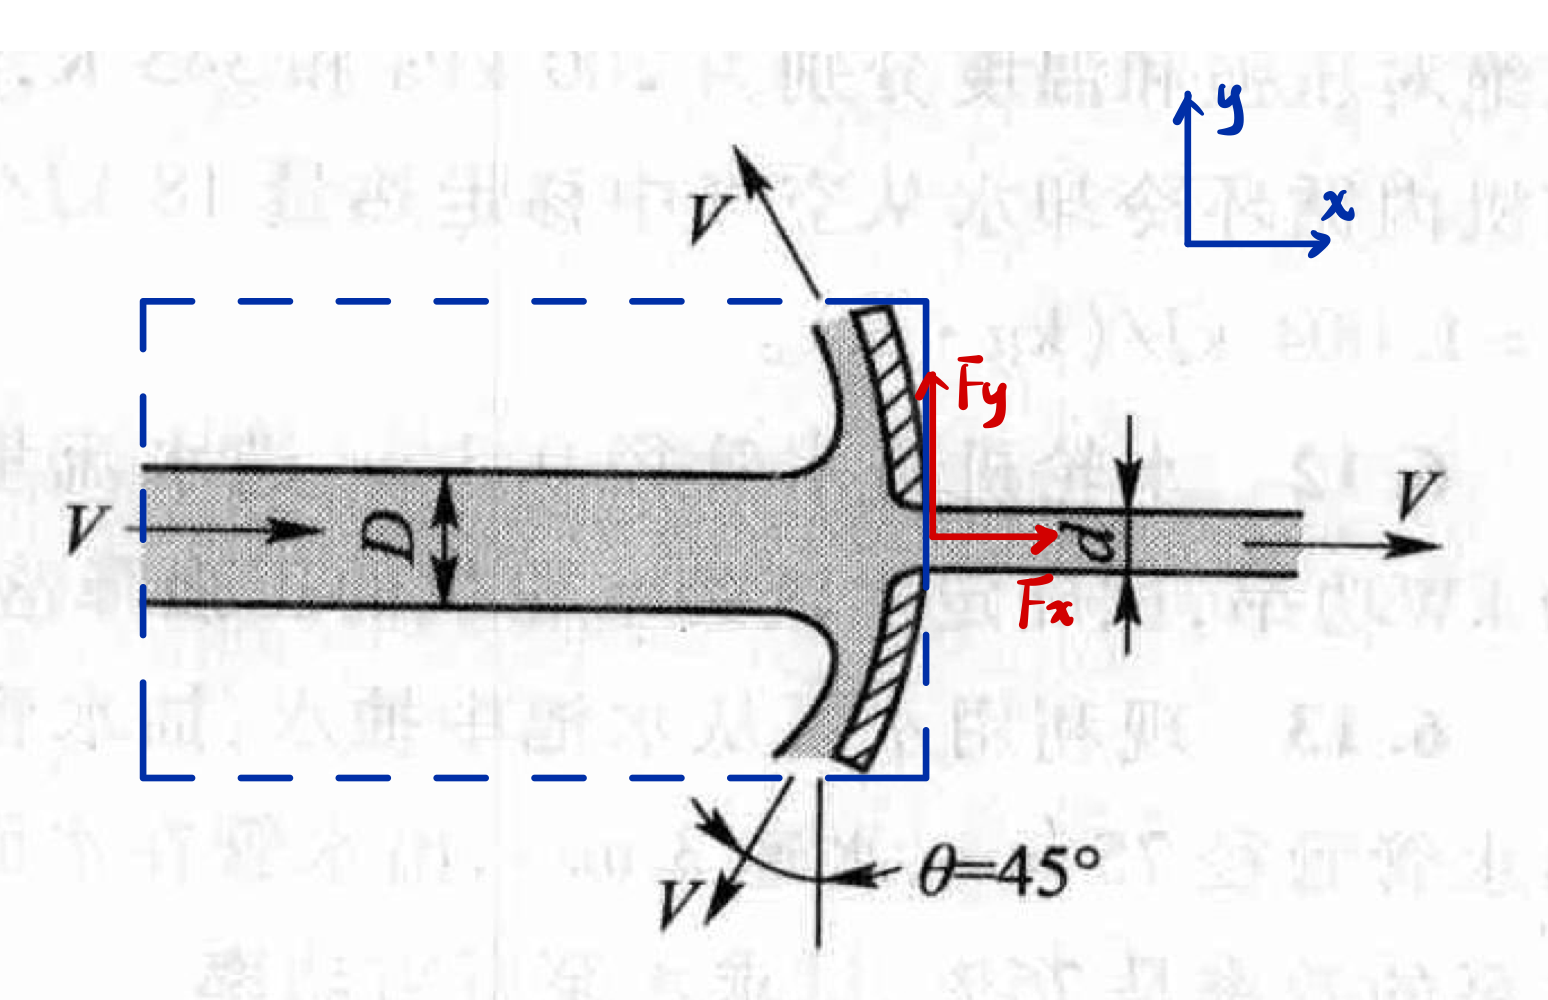
\includegraphics[scale=0.12]{figures/C6-fig3.png}
		\caption{例6.4图}
	\end{figure}
	
	设控制体上下两出口的截面积为$A_1$,根据连续方程,有
	\begin{equation*}
		V \cdot \dfrac{1}{4} \pi D^2 = 2 V \cdot A_1 + V \cdot \dfrac{1}{4} \pi d^2
	\end{equation*}
	
	解得
	\begin{equation*}
		A_1 = \dfrac{1}{8} \pi \qty(D^2 - d^2) = \dfrac{1}{8} \pi \qty(0.1^2 - 0.02^2) \mathrm{~m}^2 = 3.770 \times 10^{-3} \mathrm{~m}^2
	\end{equation*}
	
	列动量方程
	\begin{align*}
		F_x &= \sum \qty(\dot{m}_i V_{xi})_{\mathrm{out}} - \sum \qty(\dot{m}_i V_{xi})_{\mathrm{in}} \\
		&= \qty(\rho V^2 \cdot \dfrac{1}{4} \pi d^2 - 2 \rho V^2 \sin 45^{\circ} \cdot A_1) - \rho V^2 \cdot \dfrac{1}{4} \pi D^2 \\
		&= \qty(1000 \times 25 \times \dfrac{1}{4} \pi 0.02^2 - 2 \times 1000 \times \dfrac{25}{\sqrt{2}} \times 3.770 \times 10^{-3}) - 1000 \times 25 \times \dfrac{1}{4} \pi \times 0.1^2 \mathrm{~N} \\
		&= -321.8 \mathrm{~N}
	\end{align*}
	
	负号表示$F_x$方向与$x$轴正方向相反,即$F_x$的方向是水平向左。
	\begin{align*}
		F_y &= \sum \qty(\dot{m}_i V_{yi})_{\mathrm{out}} - \sum \qty(\dot{m}_i V_{yi})_{\mathrm{in}} \\
		&= \qty(\rho V^2 \cos 45^{\circ} \cdot A_1 - \rho V^2 \cos 45^{\circ} \cdot A_1) - 0 \\
		&= 0
	\end{align*}
	
	综上所述,需施加一个水平向左且大小为321.8 N的力。
\end{example}

\begin{example}
	如图,小车在射流冲击下以恒定速度$U$沿水平方向运动,固定在车上的叶片的偏转角为$\theta$。射流的绝对速度为$V$,试求叶片受到的合力及产生的功率大小,并证明$U = V/3$时该功率最大。
	
	\begin{figure}[H]
		\centering
		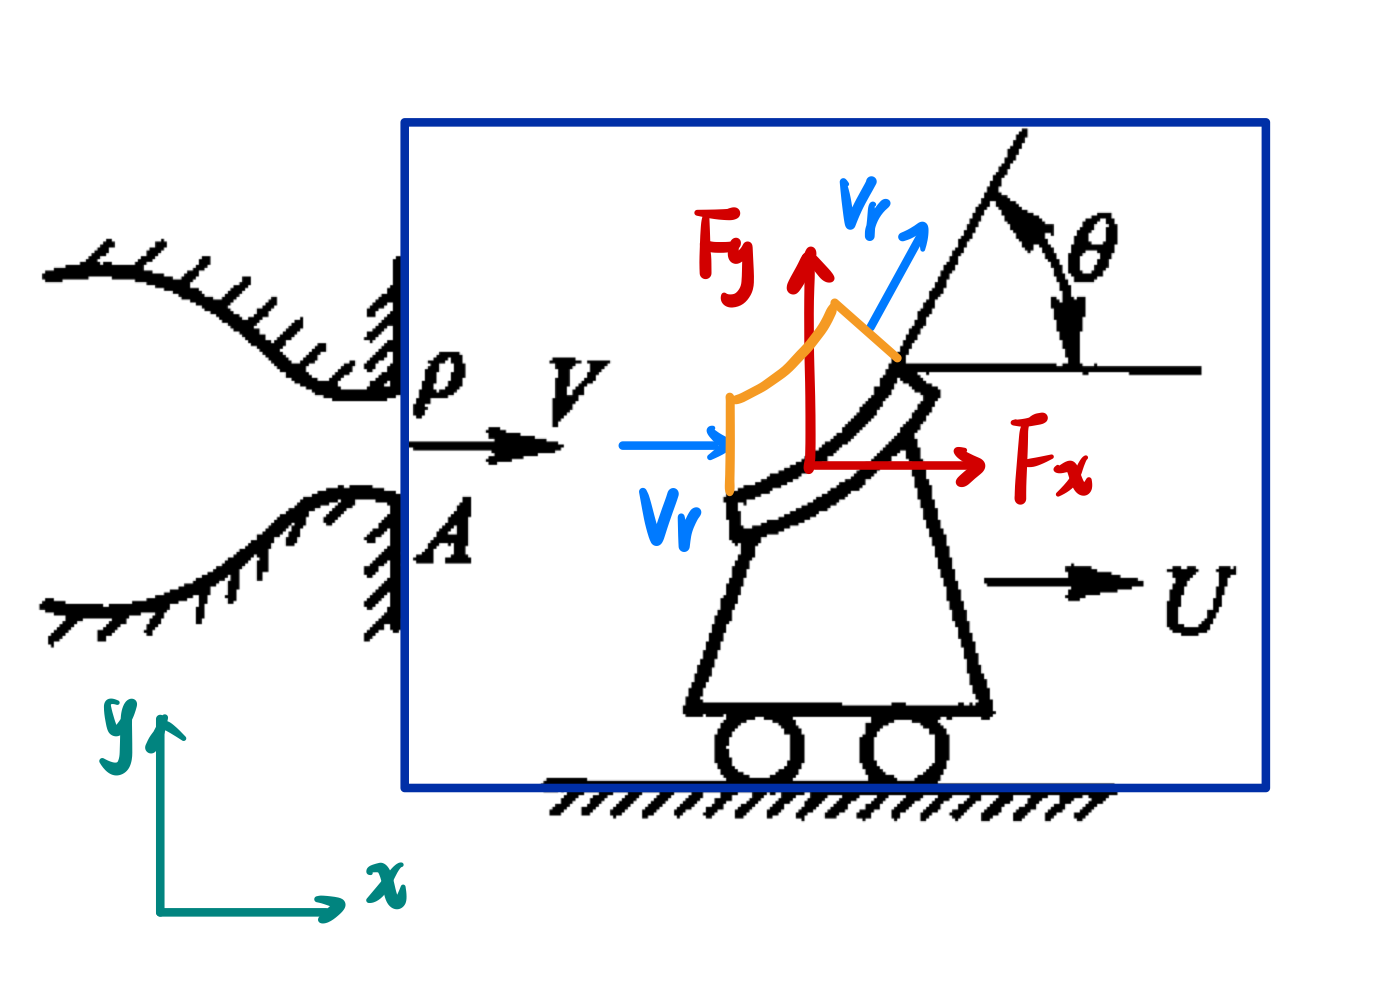
\includegraphics[scale=0.12]{figures/C6-fig2.png}
	\end{figure}

    建立如图所示的坐标系,令其相对于小车静止,则相对速度$V_r = V - U$。
    
    列动量方程
    \begin{align*}
    	&F_x = \sum \qty(\dot{m}_i V_{xi})_{\mathrm{out}} - \sum \qty(\dot{m}_i V_{xi})_{\mathrm{in}} = \rho V_r^2 \cos \theta A - \rho V_r^2 A \\
    	&F_y = \sum \qty(\dot{m}_i V_{yi})_{\mathrm{out}} - \sum \qty(\dot{m}_i V_{yi})_{\mathrm{in}} = \rho V_r^2 \sin \theta A
    \end{align*}
    
    由牛顿第三定律,得到叶片受到的力为
    \begin{align*}
    	&F_x' = \rho \qty(V-U)^2 A \qty(1-\cos \theta) \quad \text{方向水平向右} \\
    	&F_y' = -\rho \qty(V-U)^2 A \sin \theta \quad \text{方向竖直向下}
    \end{align*}
    
    产生功率
    \begin{equation*}
    	P = F_x' U = \rho \qty(V-U)^2 U A \qty(1-\cos \theta)
    \end{equation*}
    
    记$P = P\qty(U)$,则
    \begin{align*}
    	\dv{P}{U} &= \rho A \qty(1 - \cos \theta) \cdot \qty[-2\qty(V-U)U - \qty(V-U)^2] \\
    	&= \rho A \qty(1 - \cos \theta) \cdot \qty(U - V) \qty(U - \dfrac{V}{3})
    \end{align*}
    
    令$\displaystyle \dv{P}{U} = 0$,解得$U = V$或$U = V/3$。
    
    \vskip 0.3cm
    
    求二阶导数
    \begin{equation*}
    	\dv[2]{P}{U} = \rho A \qty(1 - \cos \theta) (6U - 4V)
    \end{equation*}
    
    代入两根,有
    \begin{align*}
    	&\dv[2]{P}{U} \Big|_{U=V} = 2 \rho A \qty(1 - \cos \theta) > 0,\text{~此时$P$有极小值} \\
    	&\dv[2]{P}{U} \Big|_{U=V/3} = -2 \rho A \qty(1 - \cos \theta) < 0,\text{~此时$P$有极大值}
    \end{align*}
    
    故,$U = V/3$时叶片受力产生的功率最大。
\end{example}

\begin{tip}
	考试中本章必涉及一道大题,2021年期末第2道计算大题跟\textbf{例6.4}比较相似。
\end{tip}
